%% bare_conf.tex
%% V1.4b
%% 2015/08/26
%% by Michael Shell
%% See:
%% http://www.michaelshell.org/
%% for current contact information.
%%
%% This is a skeleton file demonstrating the use of IEEEtran.cls
%% (requires IEEEtran.cls version 1.8b or later) with an IEEE
%% conference paper.
%%
%% Support sites:
%% http://www.michaelshell.org/tex/ieeetran/
%% http://www.ctan.org/pkg/ieeetran
%% and
%% http://www.ieee.org/

%%*************************************************************************
%% Legal Notice:
%% This code is offered as-is without any warranty either expressed or
%% implied; without even the implied warranty of MERCHANTABILITY or
%% FITNESS FOR A PARTICULAR PURPOSE! 
%% User assumes all risk.
%% In no event shall the IEEE or any contributor to this code be liable for
%% any damages or losses, including, but not limited to, incidental,
%% consequential, or any other damages, resulting from the use or misuse
%% of any information contained here.
%%
%% All comments are the opinions of their respective authors and are not
%% necessarily endorsed by the IEEE.
%%
%% This work is distributed under the LaTeX Project Public License (LPPL)
%% ( http://www.latex-project.org/ ) version 1.3, and may be freely used,
%% distributed and modified. A copy of the LPPL, version 1.3, is included
%% in the base LaTeX documentation of all distributions of LaTeX released
%% 2003/12/01 or later.
%% Retain all contribution notices and credits.
%% ** Modified files should be clearly indicated as such, including  **
%% ** renaming them and changing author support contact information. **
%%*************************************************************************


% *** Authors should verify (and, if needed, correct) their LaTeX system  ***
% *** with the testflow diagnostic prior to trusting their LaTeX framework ***
% *** with production work. The IEEE's font choices and paper sizes can   ***
% *** trigger bugs that do not appear when using other class files.       ***                          ***
% The testflow support page is at:
% http://www.michaelshell.org/tex/testflow/


\label{beginning of document}
\documentclass[conference]{IEEEtran}
% Some Computer Society conferences also require the compsoc mode option,
% but others use the standard conference format.
%
% If IEEEtran.cls has not been installed into the LaTeX system files,
% manually specify the path to it like:
% \documentclass[conference]{../sty/IEEEtran}

\renewcommand\IEEEkeywordsname{Keywords}
\usepackage{makeidx}  % allows for indexgeneration
\usepackage[table]{xcolor}
\usepackage{graphicx}
	\graphicspath{{images/}} 
\usepackage{cite}
\usepackage{courier}
\usepackage{hyperref}
    \hypersetup{colorlinks=true,allcolors=blue}
\usepackage{listings}
	\lstset{
  		basicstyle=\ttfamily,
  		frame=none,
  		breaklines=true,
  		numbers=left,
  		xleftmargin=2em,
  		framexleftmargin=0em,
    	emphstyle=\textbf,
    	float=t
	}
	\lstdefinestyle{ocl}{
  		emph={
        	context, inv
    	}
	}
	\lstdefinestyle{cbp}{
	    basicstyle=\ttfamily\scriptsize,
  		emph={
        	session, create, of, type,
        	set, to, add, hire
    	}
	}
	\lstdefinestyle{xmi}{
		basicstyle=\ttfamily\scriptsize,
  		emph={
        	Employee, manages
    	}
	}
	\lstdefinestyle{xml}{
	    basicstyle=\ttfamily\scriptsize,
  		emph={
        	register, create, add, to, resource,
        	from, eattribute, remove, ereference,
        	set, unset, session, Roy, Jen,
        	Moss, Richmond
    	}
	}
	\lstdefinestyle{java}{
	    basicstyle=\ttfamily\scriptsize,
  		emph={
        	case, UNSET,
        	instanceof, else, if, void,
        	new, UnsetEAttributeEvent,
        	UnsetEReferenceEvent,
        	@override, public, class, extends
    	}
	}


% Some very useful LaTeX packages include:
% (uncomment the ones you want to load)


% *** MISC UTILITY PACKAGES ***
%
%\usepackage{ifpdf}
% Heiko Oberdiek's ifpdf.sty is very useful if you need conditional
% compilation based on whether the output is pdf or dvi.
% usage:
% \ifpdf
%   % pdf code
% \else
%   % dvi code
% \fi
% The latest version of ifpdf.sty can be obtained from:
% http://www.ctan.org/pkg/ifpdf
% Also, note that IEEEtran.cls V1.7 and later provides a builtin
% \ifCLASSINFOpdf conditional that works the same way.
% When switching from latex to pdflatex and vice-versa, the compiler may
% have to be run twice to clear warning/error messages.






% *** CITATION PACKAGES ***
%
%\usepackage{cite}
% cite.sty was written by Donald Arseneau
% V1.6 and later of IEEEtran pre-defines the format of the cite.sty package
% \cite{} output to follow that of the IEEE. Loading the cite package will
% result in citation numbers being automatically sorted and properly
% "compressed/ranged". e.g., [1], [9], [2], [7], [5], [6] without using
% cite.sty will become [1], [2], [5]----[7], [9] using cite.sty. cite.sty's
% \cite will automatically add leading space, if needed. Use cite.sty's
% noadjust option (cite.sty V3.8 and later) if you want to turn this off
% such as if a citation ever needs to be enclosed in parenthesis.
% cite.sty is already installed on most LaTeX systems. Be sure and use
% version 5.0 (2009-03-20) and later if using hyperref.sty.
% The latest version can be obtained at:
% http://www.ctan.org/pkg/cite
% The documentation is contained in the cite.sty file itself.






% *** GRAPHICS RELATED PACKAGES ***
%
\ifCLASSINFOpdf
  % \usepackage[pdftex]{graphicx}
  % declare the path(s) where your graphic files are
  % \graphicspath{{../pdf/}{../jpeg/}}
  % and their extensions so you won't have to specify these with
  % every instance of \includegraphics
  % \DeclareGraphicsExtensions{.pdf,.jpeg,.png}
\else
  % or other class option (dvipsone, dvipdf, if not using dvips). graphicx
  % will default to the driver specified in the system graphics.cfg if no
  % driver is specified.
  % \usepackage[dvips]{graphicx}
  % declare the path(s) where your graphic files are
  % \graphicspath{{../eps/}}
  % and their extensions so you won't have to specify these with
  % every instance of \includegraphics
  % \DeclareGraphicsExtensions{.eps}
\fi
% graphicx was written by David Carlisle and Sebastian Rahtz. It is
% required if you want graphics, photos, etc. graphicx.sty is already
% installed on most LaTeX systems. The latest version and documentation
% can be obtained at: 
% http://www.ctan.org/pkg/graphicx
% Another good source of documentation is "Using Imported Graphics in
% LaTeX2e" by Keith Reckdahl which can be found at:
% http://www.ctan.org/pkg/epslatex
%
% latex, and pdflatex in dvi mode, support graphics in encapsulated
% postscript (.eps) format. pdflatex in pdf mode supports graphics
% in .pdf, .jpeg, .png and .mps (metapost) formats. Users should ensure
% that all non-photo figures use a vector format (.eps, .pdf, .mps) and
% not a bitmapped formats (.jpeg, .png). The IEEE frowns on bitmapped formats
% which can result in "jaggedy"/blurry rendering of lines and letters as
% well as large increases in file sizes.
%
% You can find documentation about the pdfTeX application at:
% http://www.tug.org/applications/pdftex





% *** MATH PACKAGES ***
%
%\usepackage{amsmath}
% A popular package from the American Mathematical Society that provides
% many useful and powerful commands for dealing with mathematics.
%
% Note that the amsmath package sets \interdisplaylinepenalty to 10000
% thus preventing page breaks from occurring within multiline equations. Use:
%\interdisplaylinepenalty=2500
% after loading amsmath to restore such page breaks as IEEEtran.cls normally
% does. amsmath.sty is already installed on most LaTeX systems. The latest
% version and documentation can be obtained at:
% http://www.ctan.org/pkg/amsmath





% *** SPECIALIZED LIST PACKAGES ***
%
%\usepackage{algorithmic}
% algorithmic.sty was written by Peter Williams and Rogerio Brito.
% This package provides an algorithmic environment fo describing algorithms.
% You can use the algorithmic environment in-text or within a figure
% environment to provide for a floating algorithm. Do NOT use the algorithm
% floating environment provided by algorithm.sty (by the same authors) or
% algorithm2e.sty (by Christophe Fiorio) as the IEEE does not use dedicated
% algorithm float types and packages that provide these will not provide
% correct IEEE style captions. The latest version and documentation of
% algorithmic.sty can be obtained at:
% http://www.ctan.org/pkg/algorithms
% Also of interest may be the (relatively newer and more customizable)
% algorithmicx.sty package by Szasz Janos:
% http://www.ctan.org/pkg/algorithmicx




% *** ALIGNMENT PACKAGES ***
%
%\usepackage{array}
% Frank Mittelbach's and David Carlisle's array.sty patches and improves
% the standard LaTeX2e array and tabular environments to provide better
% appearance and additional user controls. As the default LaTeX2e table
% generation code is lacking to the point of almost being broken with
% respect to the quality of the end results, all users are strongly
% advised to use an enhanced (at the very least that provided by array.sty)
% set of table tools. array.sty is already installed on most systems. The
% latest version and documentation can be obtained at:
% http://www.ctan.org/pkg/array


% IEEEtran contains the IEEEeqnarray family of commands that can be used to
% generate multiline equations as well as matrices, tables, etc., of high
% quality.




% *** SUBFIGURE PACKAGES ***
%\ifCLASSOPTIONcompsoc
%  \usepackage[caption=false,font=normalsize,labelfont=sf,textfont=sf]{subfig}
%\else
%  \usepackage[caption=false,font=footnotesize]{subfig}
%\fi
% subfig.sty, written by Steven Douglas Cochran, is the modern replacement
% for subfigure.sty, the latter of which is no longer maintained and is
% incompatible with some LaTeX packages including fixltx2e. However,
% subfig.sty requires and automatically loads Axel Sommerfeldt's caption.sty
% which will override IEEEtran.cls' handling of captions and this will result
% in non-IEEE style figure/table captions. To prevent this problem, be sure
% and invoke subfig.sty's "caption=false" package option (available since
% subfig.sty version 1.3, 2005/06/28) as this is will preserve IEEEtran.cls
% handling of captions.
% Note that the Computer Society format requires a larger sans serif font
% than the serif footnote size font used in traditional IEEE formatting
% and thus the need to invoke different subfig.sty package options depending
% on whether compsoc mode has been enabled.
%
% The latest version and documentation of subfig.sty can be obtained at:
% http://www.ctan.org/pkg/subfig




% *** FLOAT PACKAGES ***
%
%\usepackage{fixltx2e}
% fixltx2e, the successor to the earlier fix2col.sty, was written by
% Frank Mittelbach and David Carlisle. This package corrects a few problems
% in the LaTeX2e kernel, the most notable of which is that in current
% LaTeX2e releases, the ordering of single and double column floats is not
% guaranteed to be preserved. Thus, an unpatched LaTeX2e can allow a
% single column figure to be placed prior to an earlier double column
% figure.
% Be aware that LaTeX2e kernels dated 2015 and later have fixltx2e.sty's
% corrections already built into the system in which case a warning will
% be issued if an attempt is made to load fixltx2e.sty as it is no longer
% needed.
% The latest version and documentation can be found at:
% http://www.ctan.org/pkg/fixltx2e


%\usepackage{stfloats}
% stfloats.sty was written by Sigitas Tolusis. This package gives LaTeX2e
% the ability to do double column floats at the bottom of the page as well
% as the top. (e.g., "\begin{figure*}[!b]" is not normally possible in
% LaTeX2e). It also provides a command:
%\fnbelowfloat
% to enable the placement of footnotes below bottom floats (the standard
% LaTeX2e kernel puts them above bottom floats). This is an invasive package
% which rewrites many portions of the LaTeX2e float routines. It may not work
% with other packages that modify the LaTeX2e float routines. The latest
% version and documentation can be obtained at:
% http://www.ctan.org/pkg/stfloats
% Do not use the stfloats baselinefloat ability as the IEEE does not allow
% \baselineskip to stretch. Authors submitting work to the IEEE should note
% that the IEEE rarely uses double column equations and that authors should try
% to avoid such use. Do not be tempted to use the cuted.sty or midfloat.sty
% packages (also by Sigitas Tolusis) as the IEEE does not format its papers in
% such ways.
% Do not attempt to use stfloats with fixltx2e as they are incompatible.
% Instead, use Morten Hogholm'a dblfloatfix which combines the features
% of both fixltx2e and stfloats:
%
% \usepackage{dblfloatfix}
% The latest version can be found at:
% http://www.ctan.org/pkg/dblfloatfix




% *** PDF, URL AND HYPERLINK PACKAGES ***
%
%\usepackage{url}
% url.sty was written by Donald Arseneau. It provides better support for
% handling and breaking URLs. url.sty is already installed on most LaTeX
% systems. The latest version and documentation can be obtained at:
% http://www.ctan.org/pkg/url
% Basically, \url{my_url_here}.




% *** Do not adjust lengths that control margins, column widths, etc. ***
% *** Do not use packages that alter fonts (such as pslatex).         ***
% There should be no need to do such things with IEEEtran.cls V1.6 and later.
% (Unless specifically asked to do so by the journal or conference you plan
% to submit to, of course. )


% correct bad hyphenation here
\hyphenation{op-tical net-works semi-conduc-tor}


\begin{document}
\renewcommand{\thelstlisting}{\arabic{lstlisting}}
\renewcommand{\labelitemi}{$\bullet$}
\newcommand{\dk}[1]{\textbf{[DK: #1]}}
%
% paper title
% Titles are generally capitalized except for words such as a, an, and, as,
% at, but, by, for, in, nor, of, on, or, the, to and up, which are usually
% not capitalized unless they are the first or last word of the title.
% Linebreaks \\ can be used within to get better formatting as desired.
% Do not put math or special symbols in the title.
\title{Turning Models Inside Out}


% author names and affiliations
% use a multiple column layout for up to three different
% affiliations
\author{\IEEEauthorblockN{Alfa Yohannis, Dimitris Kolovos, Fiona Polack}
\IEEEauthorblockA{Department of Computer Science\\
University of York\\
York, United Kingdom\\
\{ary506, dimitris.kolovos, fiona.pollack\}@york.ac.uk}}

% conference papers do not typically use \thanks and this command
% is locked out in conference mode. If really needed, such as for
% the acknowledgment of grants, issue a \IEEEoverridecommandlockouts
% after \documentclass

% for over three affiliations, or if they all won't fit within the width
% of the page, use this alternative format:
% 
%\author{\IEEEauthorblockN{Michael Shell\IEEEauthorrefmark{1},
%Homer Simpson\IEEEauthorrefmark{2},
%James Kirk\IEEEauthorrefmark{3}, 
%Montgomery Scott\IEEEauthorrefmark{3} and
%Eldon Tyrell\IEEEauthorrefmark{4}}
%\IEEEauthorblockA{\IEEEauthorrefmark{1}School of Electrical and Computer Engineering\\
%Georgia Institute of Technology,
%Atlanta, Georgia 30332--0250\\ Email: see http://www.michaelshell.org/contact.html}
%\IEEEauthorblockA{\IEEEauthorrefmark{2}Twentieth Century Fox, Springfield, USA\\
%Email: homer@thesimpsons.com}
%\IEEEauthorblockA{\IEEEauthorrefmark{3}Starfleet Academy, San Francisco, California 96678-2391\\
%Telephone: (800) 555--1212, Fax: (888) 555--1212}
%\IEEEauthorblockA{\IEEEauthorrefmark{4}Tyrell Inc., 123 Replicant Street, Los Angeles, California 90210--4321}}




% use for special paper notices
%\IEEEspecialpapernotice{(Invited Paper)}




% make the title area
\maketitle

% As a general rule, do not put math, special symbols or citations
% in the abstract
\begin{abstract}
\label{abstract}
We present an approach for change-based (as opposed to state-based) model persistence that can facilitate high-performance incremental model processing (e.g. validation, transformation) by minimising the cost of change identification when models evolve. We illustrate a prototype that implements the proposed approach on top of the Eclipse Modelling Framework and we present a roadmap for further work in this direction.
\end{abstract}

% no keywords
\begin{IEEEkeywords} 
model-driven, persistence, incremental, change events, notification
\end{IEEEkeywords}



% For peer review papers, you can put extra information on the cover
% page as needed:
% \ifCLASSOPTIONpeerreview
% \begin{center} \bfseries EDICS Category: 3-BBND \end{center}
% \fi
%
% For peerreview papers, this IEEEtran command inserts a page break and
% creates the second title. It will be ignored for other modes.
\IEEEpeerreviewmaketitle

\section{Introduction}
\label{Introduction}
% The way we handle models nowadays are mostly based on non-incremental approach -- it persists states of models as snapshots. When the size of a model is small, the cost to process (e.g. validate, transform) the model is insignificant. Once the model becomes large, the processes turn to be cumbersome, particularly when small changes are made, but the whole model needs to be re-validated and re-transformed. To overcome this issue, several existing works \cite{egyed2011automatically, jouault2010towards, rath2012derived, ogunyomi2015property} have applied variants of incremental-based approach to improving model operation performance. The ``incremental" means the time to update the results of a model processing operation should be proportional to the size of the change of a modified model. This research aims to persist models change history as a mean to harness incremental-based approach to enable high-performance model processing operations.

% As MBSE is used for the development of larger and more complex systems in a variety of domains, the ability to process (e.g. validate, transform, generate code from) large models in an incremental fashion as they evolve becomes essential. ``Incremental'' in this context means that the amount of time it takes to update the results of a model processing operation on a modified model, is generally proportional to the size of the change, as opposed to the size of the model.

To reap the benefits of Model-Based Software Engineering in the context of large and complex systems, the ability to process large models in an incremental fashion as they evolve is essential. Current incremental model processing techniques only deliver limited performance benefits due to slow and imprecise model change detection capabilities or are limited to a single-developer environment; not realistic for real-world software development projects.

The research introduced in this paper aims at enabling flexible and high-performance incremental model processing through change-based model persistence. That is, instead of persisting snapshots of the state of models, we propose turning models inside out and persisting their change history. The proposed approach has the potential to deliver step-change performance benefits in incremental model processing, as well as a wide range of other benefits and novel capabilities.

The rest of the paper is structured as follows. Section \ref{sec:the_key_challenge_of_ _incrementality} reviews the key-challenge of incrementality in MBSE. Section \ref{sec:identifying_changes_in models} provides an overview of existing approaches for identifying changes in models. Section \ref{sec:proposed_approach} overviews our proposed approach and Section \ref{sec:prototype_implementation} discusses our prototype implementation on top of the Eclipse Modelling Framework. The potential benefits and novel capabilities, as well as the challenges of change-based model persistence, are presented in Sect. \ref{sec:benefits_and_novel_capabilities} and Sect. \ref{sec:challenges_and_future_works} respectively. Section \ref{sec:evaluation_strategy} presents our evaluation strategy and Sect. \ref{sec:conclusions} concludes this paper.

\section{The Key-Challenge of Incrementality}
\label{sec:the_key_challenge_of_ _incrementality}
%\dk{See \url{https://en.wikibooks.org/wiki/LaTeX/Labels_and_Cross-referencing} for naming conventions for LaTeX labels}
To illustrate the concept of incrementality, a contrived running example is used where after every modification to an organisational chart model (see Fig. \ref{fig:initial_chart}), the model needs to be:

\begin{itemize}
\item Validated against a domain-specific constraint (that no employee directly manages more than 7 other employees).
\item Transformed into a number of employee reports (plain text files, one for each employee) through a model-to-text transformation. Each report should contain the name of the employee, and the names of her direct subordinates.
\end{itemize}

Figures \ref{fig:initial_chart} and \ref{fig:modified_chart} are two consecutive versions of a sample organisational chart model. When the validation constraint is evaluated against the first version of the model (Fig. \ref{fig:initial_chart}), it verifies that all three employees manage fewer than 7 other employees, and the model-to-text transformation then produces three text files that correspond to the employees in the model. In the sequel, in Fig. \ref{fig:modified_chart}, the model is updated to reflect that a new employee has been hired (Richmond) under the management of Jen. 

\begin{figure}[ht]
\centering
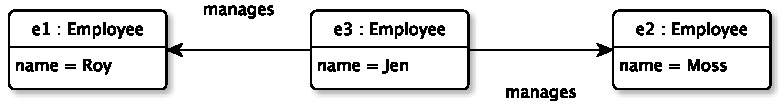
\includegraphics[width=\linewidth]{initial_chart}
\caption{Initial version of the organisational chart model.}
\label{fig:initial_chart}
\end{figure}

\begin{figure}[ht]
\centering
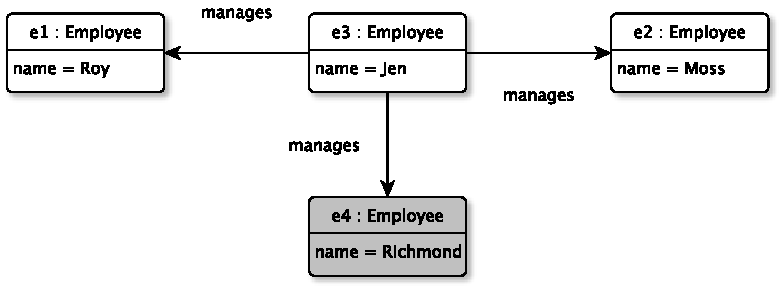
\includegraphics[width=\linewidth]{modified_chart}
\caption{Modified version of the organisational chart model of Fig. \ref{fig:initial_chart}.}
\label{fig:modified_chart}
\end{figure}

A non-incremental model validation engine would treat the model of Fig. \ref{fig:modified_chart} as if it was a new model and would evaluate the constraint above against every employee in the model. An incremental model validation engine, on the other hand, would identify that the previously established satisfaction of the constraint for employees Moss and Roy cannot have been possibly compromised by the changes made, and would only re-evaluate the constraint for Jen and Richmond instead. 

Similarly, a non-incremental model-to-text transformation would generate and overwrite all employee reports from scratch. On the contrary, an incremental model-to-text transformation, would identify that it only needs to generate a new report for the new employee (Richmond), and to recompute and overwrite the contents of Jen's report (as she is now managing an additional employee)---but not the reports of Moss or Roy, as these cannot have been affected by the changes made to the model.

While the overhead of executing transformations and validation constraints on small models like the one in Fig. \ref{fig:modified_chart} is negligible, non-incremental execution can become a significant bottleneck for large evolving models. As stressed in Selic's seminal work \cite{selic2003pragmatics}, with reference to model-to-text transformation, ``... \emph{this is particularly true in the latter phases of the development cycle when programmers make many small changes as they fine-tune the system. To keep this overhead low, it is crucial for the code generators to have sophisticated change impact analysis capabilities that minimize the amount of code regeneration}".

As demonstrated by the pioneering work of Egyed \cite{egyed2011automatically}, to achieve incremental re-execution of (deterministic) queries on structured models, an execution engine needs to:

\begin{enumerate}
\item Record model element property accesses during the initial execution of the queries;
\item Identify new and deleted elements and modified model element properties in the new version of the model;
\item Combine the information collected in the steps above to identify the subset of (potentially) affected rules/queries/templates that need to be re-executed.
\end{enumerate}

To illustrate this, we use an OCL implementation of the domain-specific constraint in List. \ref{lst:constraint}.

\begin{lstlisting}[style=ocl,caption={OCL constraint requiring that no employee directly manages more than 7 other employees.},label=lst:constraint]
context Employee
inv NoMoreThan7: self.manages->size() <= 7
\end{lstlisting}

During the initial evaluation of the constraint on the model of Fig. \ref{fig:initial_chart}, an incremental OCL engine would compute the property access trace displayed in Table \ref{tab:property_access_trace} as a side-product. Now, when the model is updated (Fig. \ref{fig:modified_chart}), the execution engine can identify that:

\begin{itemize}
\item There is new element in the model (\emph{e4} - Richmond) for which the constraint has not been evaluated;
\item The value of the manages property of Jen (\emph{e3}) has changed, and as such, it needs to re-evaluate the constraint on this model-element.
\end{itemize}

\begin{table}[htbp]
\centering
\caption{Property-access trace of the evaluation of the constraint in List. \ref{lst:constraint} on the model of Fig. \ref{fig:initial_chart}.}
\begin{tabular}{p{0.35\linewidth} p{0.15\linewidth} p{0.15\linewidth} p{0.15\linewidth}}
\hline 
\textbf{Constraint} & \textbf{Context} & \textbf{Accessed Element} & \textbf{Accessed Property} \\ 
\hline 
\emph{Employee.NoMoreThan7}  & \emph{e1} & \emph{e1} & \emph{manages} \\ 
\emph{Employee.NoMoreThan7}  & \emph{e2} & \emph{e2} & \emph{manages} \\ 
\emph{Employee.NoMoreThan7}  & \emph{e3} & \emph{e3} & \emph{manages} \\ 
\hline 
\end{tabular} 
\label{tab:property_access_trace}
\end{table}

Egyed has shown that the property-access recording approach is applicable to queries of arbitrary complexity, as long as they are deterministic. More recent work has shown that variants of this approach can be used to achieve incrementality in a wide range of model processing operations, including model-to-model transformation \cite{jouault2010towards}, model-to-text transformation \cite{ogunyomi2015property}, model validation, and pattern matching \cite{rath2012derived}---as long as changes to models can be precisely identified (step 2 in the list above).

\section{Identifying Changes in Models}
\label{sec:identifying_changes_in models}
There are two approaches in the literature for identifying changes in models in order to enable incremental re-execution of model processing operations.

\textbf{Notifications}. In this approach, the incremental execution engine needs to hook into the notification facilities provided by the modelling tool through which the developer edits the model, so that the engine can directly receive notifications as soon as changes happen (e.g. a new employee (\emph{e4}) has been added, the name property of employee \emph{e4} has been changed to ``Richmond"). This is an approach taken by the IncQuery incremental pattern matching framework \cite{rath2012derived} and the ReactiveATL incremental model-to-model transformation engine \cite{ogunyomi2015property}. The main advantage of this approach is that precise and fine-grained change notifications are provided for free by the modelling tool (and thus do not need to be computed by the execution engine---which as discussed below can be expensive and inefficient). On the downside, this approach is a poor fit for collaborative development settings where modelling and automated model processing activities are performed by different members of the team.

\begin{figure*}[h]
\begin{lstlisting}[style=xml,caption={Change-based representation of the model of Figure \ref{fig:modified_chart}.},label=lst:cbpmodel]
<session id="s1"/>
<create eclass="Employee" epackage="employee" id="0"/>
<add-to-resource position="0"><value eobject="0"/></add-to-resource>
<set-eattribute name="name" target="0"><value literal="Roy"/></set-eattribute>
<create eclass="Employee" epackage="employee" id="1"/>
<add-to-resource position="1"><value eobject="1"/></add-to-resource>
<set-eattribute name="name" target="1"><value literal="Jen"/></set-eattribute>
<create eclass="Employee" epackage="employee" id="2"/>
<add-to-resource position="2"><value eobject="2"/></add-to-resource>
<set-eattribute name="name" target="1"><value literal="Moss"/></set-eattribute>
<remove-from-resource><value eobject="0"/></remove-from-resource>
<add-to-ereference name="manages" position="0" target="1"><value eobject="0"/></add-to-ereference>
<remove-from-resource><value eobject="2"/></remove-from-resource>
<add-to-ereference name="manages" position="1" target="1"><value eobject="2"/></add-to-ereference>
<session id="s2"/>
<create eclass="Employee" epackage="employee" id="3"/>
<add-to-resource position="1"><value eobject="3"/></add-to-resource>
<set-eattribute name="name" target="3"><value literal="Richmond"/></set-eattribute>
<remove-from-resource><value eobject="3"/></remove-from-resource>
<add-to-ereference name="manages" position="2" target="2"><value eobject="3"/></add-to-ereference>
\end{lstlisting}
\end{figure*}

\textbf{Model Differencing}. This approach eliminates the coupling between modelling tools and incremental execution engines. Instead of depending on live notifications, in this approach the developer in charge of automated model processing, needs to have access to a copy of the last version of the model that the model processing program (e.g. the model-to-text transformation) was executed upon, so that it can be compared against the current version of the model (e.g. using a model-differencing framework such as SiDiff \cite{kelter2005generic} or EMFCompare\footnote{\url{https://www.eclipse.org/emf/compare/}}) and the delta can be computed on demand. The main advantage of this approach is that it works well in a collaborative development environment where typically developers have distinct roles and responsibilities. On the downside, model comparison and differencing are computationally expensive and memory-greedy (both versions of the model need to be loaded into memory before they can be compared), thus largely undermining the time and resource saving potentials of incremental re-execution. This approach is adopted by the Xpand model-to-text transformation language. According to the developers of the language, using this approach, a speed-up of only around 50\% is observed compared to non-incremental transformation\footnote{\url{http://wiki.eclipse.org/Xpand/New_And_Noteworthy\#Incremental_Generation}}, which is consistent with our experience from using Xpand.

In summary, incremental model processing currently delivers significant performance benefits only in a single-developer environment where the modeller is also responsible for performing all the (incremental) model processing operations. As a result, in collaborative development environments, developers need to either forgo incremental model processing altogether or to work around this limitation by manually steering model processing programs to process only subsets of their models, which is cumbersome and error prone.

\section{Proposed Approach}
\label{sec:proposed_approach}
The ambition of this research is to enable high-performance incremental model management in collaborative software development environments by challenging one of the fundamental assumptions of contemporary modelling frameworks and tools: as opposed to persisting snapshots of the state of models (which is what virtually all modelling tools and frameworks currently do), we propose turning models inside out and persisting their change history instead.

\begin{lstlisting}[style=xmi,caption={State-based representation of the model of Figure \ref{fig:modified_chart} in (simplified) XMI.},label=lst:xmimodel]
<Employee xmi:id="e2" name="Jen">
  <manages xmi:id="e1" name="Roy"/>
  <manages xmi:id="e3" name="Moss"/>
  <manages xmi:id="e4" name="Richmond"/>
</Employee>
\end{lstlisting}

To illustrate the proposed approach, List. \ref{lst:xmimodel} shows a state-based representation of the model of Fig. \ref{fig:modified_chart} in (simplified) XMI, and List. \ref{lst:cbpmodel} shows the proposed equivalent change-based representation of the same model. Instead of a snapshot of the state of the model, the representation of List. \ref{lst:cbpmodel} captures the complete sequence of change events (create/set/add/remove/delete) that were performed on the model since its creation, organised in editing sessions (2 editing sessions in the case of this model). Replaying these changes produces the same state as the one captured in List. \ref{lst:xmimodel}, so the proposed representation carries at least as much information as the state-based representation.

Such a representation is particularly suitable for incremental model processing. For example, if the model-to-text transformation discussed above ``remembers" that in its previous invocation it had processed up to editing session \emph{s1} of the model, it can readily identify the changes that have been made to the model since then (i.e. in session \emph{s2} –- lines 15-20) instead of having to rediscover them through (expensive) state-based model differencing.

\section{Prototype Implementation}
\label{sec:prototype_implementation}
We have implemented a prototype\footnote{The prototype is available under \url{https://github.com/epsilonlabs/emf-cbp}.} of the change-based model persistence format using the notification facilities provided by the Eclipse Modelling Framework. In our implementation we use the \emph{ChangeEventAdapter} class, a subclass of EMF's \emph{EContentAdapter}\footnote{\url{http://download.eclipse.org/modeling/emf/emf/javadoc/2.11/org/eclipse/emf/ecore/util/EContentAdapter.html}}, to receive and record \emph{Notification}\footnote{\url{http://download.eclipse.org/modeling/emf/emf/javadoc/2.11/org/eclipse/emf/common/notify/Notification.html}} events produced by the framework for every model-element level change.

Since not all change events are relevant to change-based persistence (e.g. EMF also produces change notifications when listeners are added/removed from the model), we have defined a set of event classes to represent events of interest. The event classes are depicted in Fig. \ref{fig:events} as subclasses of the \emph{ChangeEvent} abstract class.  %In Fig. \ref{events}, unlike other event classes,\emph{RegisterEPackageEvent} class has a reference to \emph{ChangeEventAdapater} class since the \emph{RegisterEPackageEvent} holds the information of \emph{EPackage}'s name (List. \ref{cbpmodel1}, line 3) required by the \emph{ChangeEventAdapter} to recreate a model in a de-serialisation process. 

\begin{figure}[htbh]
\centering
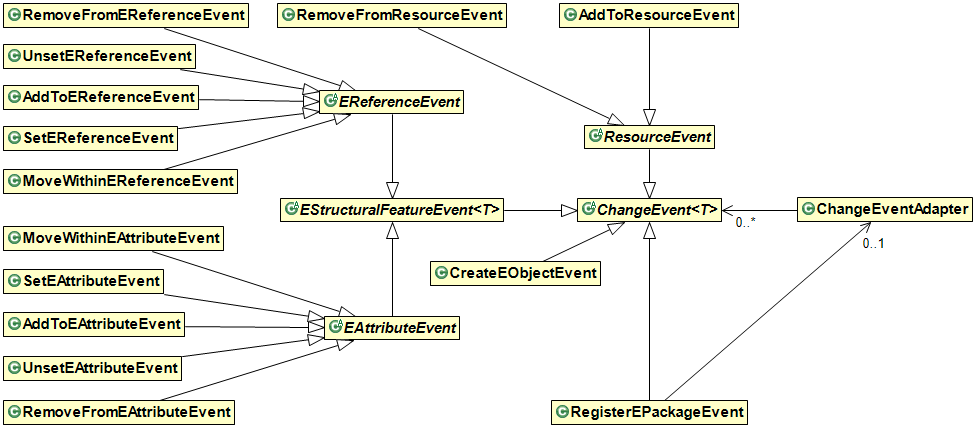
\includegraphics[width=\linewidth]{events}
\caption{Event classes to represent changes of models.}
%\dk{It would be useful to redraw the diagram so that important properties are visible (e.g. an AddToEReference event has an ``index'' and a ``value'') and also to discuss events - particularly those that may not immediately make sense to the reader (e.g. AddToResourceEvent, RegisterEPackageEvent)}
\label{fig:events}
\end{figure}

The \emph{ChangeEvent} class has a mutli-valued \emph{values} attribute which can accommodate both single-valued (e.g. set/add) or mutli-valued events (e.g. addAll/removeAll). \emph{ChangeEvent} can also accommodate different types of values, such as \emph{EObject}s for \emph{EReferenceEvents}, and primitive values (e.g. Integer, String) for \emph{EAttributeEvents}. The \emph{ChangeEvent} class also has a position attribute to hold the  index of an \emph{EObject} or a literal when they are added to a \emph{Resource}, \emph{EReference}, or \emph{EAttribute} with multiple values (Lst. \ref{lst:cbpmodel}, line 3, 6, 9, 12, 14, 17, 20). 

%When an event happens, it can involve multiple instances of \emph{EObject}. In  Lst. \ref{lst:cbpmodel} line 21, when \emph{e4} is added as an employee that \emph{e2} manages (\emph{AddToEReferenceEvent}), the \emph{e4}, \emph{manages}, and \emph{e2} are set as the event's \emph{value}, \emph{eStructuralFeature} (in this case \emph{name}), and \emph{target} respectively. The \emph{eStructuralFeature} and \emph{target} attributes are defined in the \emph{EStructuralFeatureEvent} class, which are inherited by \emph{EReferenceEvent} and \emph{EAttributeEvent} and all their subclasses (Fig. \ref{fig:events}).  

% The \emph{RegisterEPackageEvent} class is responsible to capture an event when the EMF's \emph{EPackage} of a model is registered to the \emph{ChangeEventAdapter}'s \emph{ePackages} attribute (Fig. \ref{fig:events} and Lst. \ref{lst:cbpmodel}, line 2). The information of the \emph{EPackage} is required in further model creation (e.g. create model from XML-formatted representation). The \emph{ChangeEventAdapter}'s is designed to handle multiple packages of models.

Every time an \emph{EObject} is added to the model, a \emph{CreateEObjectEvent} and an \emph{AddToResourceEvent} are recorded (lines 2-3, 5-6, 8-9, and 16-17 in Lst. \ref{lst:cbpmodel}). When an EObject is deleted, or moved to a containment \emph{EReference} deeper in the model (Lst. \ref{lst:cbpmodel}, line 12, 14, 20), a \emph{RemoveFromResourceEvent} (Lst. \ref{lst:cbpmodel}, line 11, 13, 19) is recorded.

The \emph{ChangeEventAdapter} receives EMF change notifications in its \emph{notifyChanged()} method and filters and transforms them into appropriate change events. As an example of how notifications are filtered and transformed, Listing \ref{lst:javacode} shows how we handle \emph{Notification.UNSET} events based on the type of the changed feature i.e. an \emph{UnsetEAttributeEvent} is instantiated if the feature of the notifier is an \emph{EAttribute}, or an \emph{UnsetEReferenceEvent}  is created if the notifier is an \emph{EReference}. The transformed instances are then stored into a list of events in \emph{ChangeEventAdapter} (\emph{changeEvents}) for persistence. 

\begin{lstlisting}[style=java,caption={Simplified Java code to handle notification events.},label=lst:javacode]
public class ChangeEventAdapter extends EContentAdapter {
...
@override
public void notifyChanged(Notification n) {
  ...
  switch (n.getEventType()) {
    ... // other events
    case Notification.UNSET: {
    if (n.getNotifier() instanceof EObject) {
      EStructuralFeature feature = (EStructuralFeature) n.getFeature();
        if (feature instanceof EAttribute) {
            event = new UnsetEAttributeEvent();
          } else if (feature instanceof EReference) {
            event = new UnsetEReferenceEvent();
          }
      } break;
    } 
    ... // other events
\end{lstlisting}	

To integrate seamlessly with the EMF framework and to eventually support multiple concrete change-based serialisation formats (e.g. XML-formatted representation for readability and binary for performance/size), we have created the \emph{CBPResource} abstract class, that extends EMF's built-in \emph{ResourceImpl} class. The role of the abstract class is to encapsulate all change recording functionality while the role of its concrete subclasses is to implement serialisation and de-serialisation. For example, \emph{CBPXMLResourceImpl} persists changes in a line-based format where every change is serialised as a single-line XML document. In this way, when a model changes, we can append the new changes to the end of the model file without needing to serialise the entire model again. We have also implemented a \emph{CBPXMLResourceFactory} class that extends EMF's \emph{ResourceFactoryImpl}, as the factory class for change-based models. Figure \ref{fig:resources} shows the relationships between these classes.

%The \emph{CBPXMLResourceImpl} uses an instance of \emph{ChangeEventAdapater} class to obtain a list of change events. The relationships of these classes are depicted in Fig. \ref{fig:resources}. By overriding \emph{CBPResource}'s \emph{doSave} and  \emph{doLoad} methods, we can perform serialization of the event list into an XML-formatted file and load it back again later. The representation is not a valid, complete XML format since it has no root node. Instead, it is a list of XML-formatted lines so that changes can be saved by appending new lines to the file to improve performance.


\begin{figure}[th]
\centering
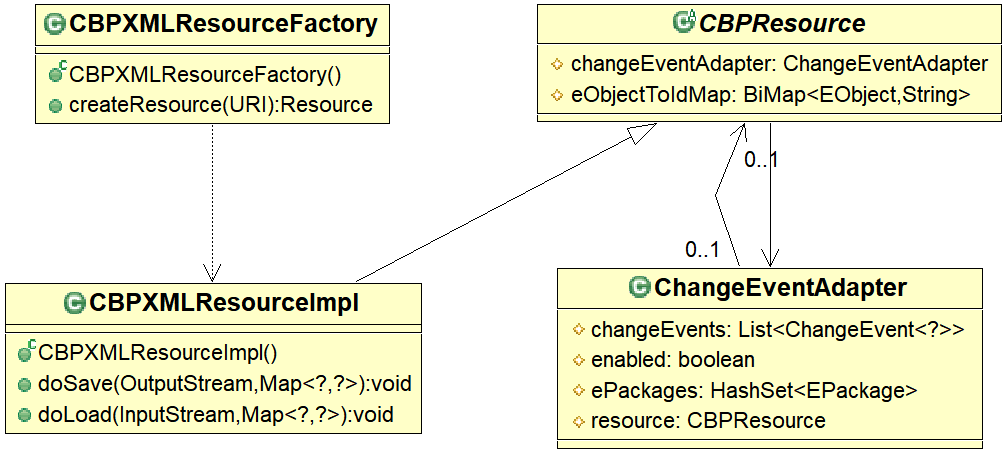
\includegraphics[scale=0.32]{resources}
\caption{Factory, resources, and ChangeEventAdapter classes.}
%\dk{See previous comment on redrawing. In its current form the diagram can be interpreted as stating that a CBPXMLResourceFactory ``has a'' CBPXMLResourceImpl, which is incorrect.}
\label{fig:resources}
\end{figure}

\section{Benefits and Novel Capabilities}
\label{sec:benefits_and_novel_capabilities}
Beyond facilitating incremental processing, the proposed representation also has the potential to deliver a wide range of benefits and novel capabilities, compared to the currently prevalent state-based representations, some of which are discussed below.

\begin{itemize}
\item With appropriate tool support, modellers will be able to ``replay" (part of) the change history of a model (e.g. to understand design decisions made by other developers, for training purposes). In state-based approaches, this can be partly achieved if models are stored in a version-control repository (e.g. Git). However, the granularity would only be at the commit level.
\item By analysing models serialised in the proposed representation, modelling language and tool vendors will be able to develop deeper insights into how modellers actually use these languages/tools in practice and utilise this information to guide the evolution of the language/tool.
\item By attaching additional information to each session (e.g. the id of the developer, references to external documents/URLs), sequences of changes can be traced back to the developer that made them, or to requirements/bug reports that triggered them.
\item Persisting changes to large models after an editing session will be significantly faster compared to serialising the entire state of the model, as only changes made during the session will need to be appended to the model file.
\item The performance and precision of model comparison and merging can be substantially improved, particularly for large models with shared editing histories.
\end{itemize}

\section{Challenges and Future Work}
\label{sec:challenges_and_future_works}
The proposed approach also comes with a number of challenges that this research will need to overcome.

\textbf{Loading Overhead}. While, as discussed above, persisting changes to large models is expected to be much faster and resource-efficient compared to state-based approaches, loading models into memory by naively replaying the entire change history is expected to have a significant overhead. To address this challenge, we will develop dedicated algorithms and data structures that will reduce the cost of change-based model loading (e.g. by recording and ignoring events -- events that are later overridden or cancelled out by other events). 

\textbf{Fast-Growing Model Files}. Persisting models in a change-based format means that model files will keep growing in size during their evolution significantly faster than their state-based counterparts. To address this challenge, (1) we will propose sound change-compression operations (e.g. remove older/unused information) that can be used to reduce the size of a model in a controlled way. (2) We will develop a compact textual format that will minimise the amount of space required to record a change (a textual line-separated format is desirable to maintain compatibility with file-based version control systems). (3) We will propose a hybrid model persistence format which will be able to incorporate both change-based and state-based information. 

\section{Evaluation Strategy}
\label{sec:evaluation_strategy}
The findings of the research will be evaluated in the small in the context of the tasks in which they will be developed, and in the large through industrial case studies. For the first type of evaluation (in the small), where there are existing approaches that the algorithms and tools developed in this research seek to outperform (e.g. change-based incremental validation vs. state-based incremental validation), comparative evaluation will be conducted to assess the benefits and limitations of our approaches. For algorithms and tools that have no direct competitors in the literature, their contributions will be assessed in comparison to the baseline they seek to improve (e.g. in this case, persisting full change histories). %Evaluation in the large will be conducted through appropriate case studies in collaboration with industrial peers.

\section{Conclusions}
\label{sec:conclusions}
Through turning models inside out and persisting their change history, this research aims at enabling high-performance incremental model processing in collaborative development settings. The proposed approach also has the potential to enable model analytics, more fine-grained tracing and to improve the precision and performance of model comparison and merging. A prototype implementation of a change-based persistence format has been presented, the main envisioned challenges have been listed and an evaluation strategy has been outlined. %Several future works also have been defined to tackle the identified challenges in realising the change-based model. Comparative evaluation will be conducted to assess the benefits and limitation of our approaches by comparing them to existing algorithms, tools, or baselines that they seek to improve.


% An example of a floating figure using the graphicx package.
% Note that \label must occur AFTER (or within) \caption.
% For figures, \caption should occur after the \includegraphics.
% Note that IEEEtran v1.7 and later has special internal code that
% is designed to preserve the operation of \label within \caption
% even when the captionsoff option is in effect. However, because
% of issues like this, it may be the safest practice to put all your
% \label just after \caption rather than within \caption{}.
%
% Reminder: the "draftcls" or "draftclsnofoot", not "draft", class
% option should be used if it is desired that the figures are to be
% displayed while in draft mode.
%
%\begin{figure}[!t]
%\centering
%\includegraphics[width=2.5in]{myfigure}
% where an .eps filename suffix will be assumed under latex, 
% and a .pdf suffix will be assumed for pdflatex; or what has been declared
% via \DeclareGraphicsExtensions.
%\caption{Simulation results for the network.}
%\label{fig_sim}
%\end{figure}

% Note that the IEEE typically puts floats only at the top, even when this
% results in a large percentage of a column being occupied by floats.


% An example of a double column floating figure using two subfigures.
% (The subfig.sty package must be loaded for this to work.)
% The subfigure \label commands are set within each subfloat command,
% and the \label for the overall figure must come after \caption.
% \hfil is used as a separator to get equal spacing.
% Watch out that the combined width of all the subfigures on a 
% line do not exceed the text width or a line break will occur.
%
%\begin{figure\\}[!t]
%\centering
%\subfloat[Case I]{\includegraphics[width=2.5in]{box}%
%\label{fig_first_case}}
%\hfil
%\subfloat[Case II]{\includegraphics[width=2.5in]{box}%
%\label{fig_second_case}}
%\caption{Simulation results for the network.}
%\label{fig_sim}
%\end{figure\\}
%
% Note that often IEEE papers with subfigures do not employ subfigure
% captions (using the optional argument to \subfloat[]), but instead will
% reference/describe all of them (a), (b), etc., within the main caption.
% Be aware that for subfig.sty to generate the (a), (b), etc., subfigure
% labels, the optional argument to \subfloat must be present. If a
% subcaption is not desired, just leave its contents blank,
% e.g., \subfloat[].


% An example of a floating table. Note that, for IEEE style tables, the
% \caption command should come BEFORE the table and, given that table
% captions serve much like titles, are usually capitalized except for words
% such as a, an, and, as, at, but, by, for, in, nor, of, on, or, the, to
% and up, which are usually not capitalized unless they are the first or
% last word of the caption. Table text will default to \footnotesize as
% the IEEE normally uses this smaller font for tables.
% The \label must come after \caption as always.
%
%\begin{table}[!t]
%% increase table row spacing, adjust to taste
%\renewcommand{\arraystretch}{1.3}
% if using array.sty, it might be a good idea to tweak the value of
% \extrarowheight as needed to properly center the text within the cells
%\caption{An Example of a Table}
%\label{table_example}
%\centering
%% Some packages, such as MDW tools, offer better commands for making tables
%% than the plain LaTeX2e tabular which is used here.
%\begin{tabular}{|c||c|}
%\hline
%One & Two\\
%\hline
%Three & Four\\
%\hline
%\end{tabular}
%\end{table}


% Note that the IEEE does not put floats in the very first column
% - or typically anywhere on the first page for that matter. Also,
% in-text middle ("here") positioning is typically not used, but it
% is allowed and encouraged for Computer Society conferences (but
% not Computer Society journals). Most IEEE journals/conferences use
% top floats exclusively. 
% Note that, LaTeX2e, unlike IEEE journals/conferences, places
% footnotes above bottom floats. This can be corrected via the
% \fnbelowfloat command of the stfloats package.



% conference papers do not normally have an appendix


% use section\\ for acknowledgment
\section*{Acknowledgments}
This work was partly supported through a scholarship managed by \emph{Lembaga Pengelola Dana Pendidikan Indonesia} (Indonesia Endowment Fund for Education).

% trigger a \newpage just before the given reference
% number - used to balance the columns on the last page
% adjust value as needed - may need to be readjusted if
% the document is modified later
%\IEEEtriggeratref{8}
% The "triggered" command can be changed if desired:
%\IEEEtriggercmd{\enlargethispage{-5in}}

% references section

% can use a bibliography generated by BibTeX as a .bbl file
% BibTeX documentation can be easily obtained at:
% http://mirror.ctan.org/biblio/bibtex/contrib/doc/
% The IEEEtran BibTeX style support page is at:
% http://www.michaelshell.org/tex/ieeetran/bibtex/
%\bibliographystyle{IEEEtran}
% argument is your BibTeX string definitions and bibliography database(s)
%\bibliography{IEEEabrv,../bib/paper}
%
% <OR> manually copy in the resultant .bbl file
% set second argument of \begin to the number of references
% (used to reserve space for the reference number labels box)
%\begin{thebibliography}{1}
%
%\bibitem{IEEEhowto:kopka}
%H.~Kopka and P.~W. Daly, \emph{A Guide to \LaTeX}, 3rd~ed.\hskip 1em plus
%  0.5em minus 0.4em\relax Harlow, England: Addison-Wesley, 1999.
%
%\end{thebibliography}

\bibliographystyle{IEEEtran}
\bibliography{references}



% that's all folks
\end{document}